\documentclass[[10pt,a4paper]{article}
\usepackage[OT4]{polski}
\usepackage[utf8]{inputenc} 
\usepackage[left=25mm,right=25mm, top=20mm, bottom = 20mm]{geometry}
\usepackage{graphicx}
\usepackage[]{mcode}
\usepackage{amsmath}
\usepackage{caption}

\graphicspath{{obrazy/}}

\begin{document}
\title{Raport końcowy projektu z przedmiotu Dedykowane Algorytmy Diagnostyki Medycznej}
\author{>autorzy<}
\date{12 stycznia 2017}
\maketitle


\begin{center}

\includegraphics{logo_agh}\\
\vspace{20mm}
{\LARGE Klasyfikacja uderzeń serca}\\

\end{center}

\newpage
\tableofcontents
\vspace{10mm}
\newpage
\section{Linear SVM}
\subsection{Opis algorytmu}
\vspace{5mm}
\subsubsection{Metoda wektorów wspierających (SVM)}
\vspace{5mm}


Maszyny wektorów wspierających (support vector machines) są modelami uczenia nadzorowanego, które analizują dane użyte do klasyfikacji i analizy regresji.
 Wykorzystując zbiór danych uczących, każdy odpowiednio oznaczony zgodnie z klasą do której przynależy, algorytm SVM tworzy model, który potrafi
przyporządkować analizowane dane do jednej z kategorii. 
\vspace{5mm}


Model SVM jest reprezentacją danych w postaci punktów w przestrzeni. Punkty należące do różnych klas znajdują się w innych obszarach przestrzeni i są rozdzielone za pomocą luki o jak największej możliwej szerokości. Kolejno, analizowany nowy punkt jest odpowiednio przyporządkowywany do jednej z kategorii na podstawie tego, z której strony luki się znajduje. Na rysunku nr 1 został przedstawiony rozkład punktów płaszczyzny należących do dwóch różnych kategorii. W tym wypadku na osiach znajdują się cechy, dzięki którym klasyfikowane są analizowane przypadki.
\vspace{5mm}
\begin{figure}[h]
\centering
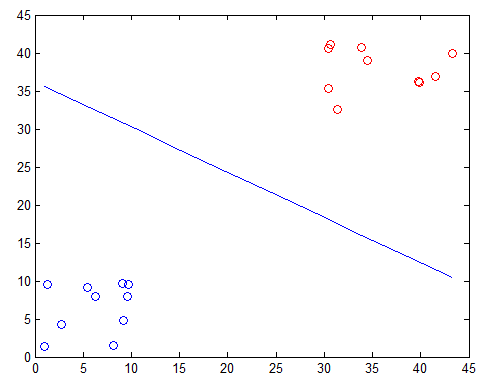
\includegraphics{svm_theory}\\
\caption{Wizualizacja punktów należących do dwóch klas wraz z rozdzielającą je hiperpłaszczyzną} 
\textit{(opracowanie własne)}
\end{figure}

\vspace{10mm}
Klasyfikacja danych jest najważniejszym zadaniem uczenia maszynowego. W metodzie wektorów wspierających dane są postaci wektora o rozmiarze $p$. Celem działania algorytmu jest wyznaczenie optymalnej hiperpłaszczyzny rozmiaru $p-1$, która rozdzielałaby dane należące do poszczególnych klas.
Tego typu podejście jest nazywane klasyfikacją liniową. 
\vspace{5mm}


\indent Istnieje wiele hiperpłaszczyzn, które mogą rozdzielać dwie klasy. Przykładowo na rysunku 2 przedstawiono dwie klasy rozdzielone trzema różnymi hiperpłaszczyznami $H_1, H_2, H_3$. Problem polega na tym, aby wybrać jak najlepszą hiperpłaszczyznę, która w sposób najbardziej optymalny będzie rozdzielać dwie klasy. Taka hiperpłaszczyzna zostaje wybrana w taki sposób, aby była jak najbardziej oddalona zarówno od jednej jak i drugiej klasy. 


\begin{figure}[h]
\centering
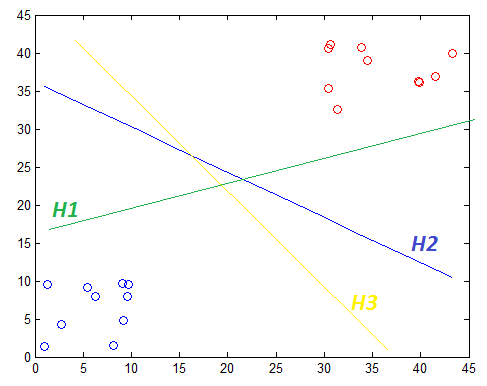
\includegraphics{svm_hyperplane}\\
\caption{Wizualizacja trzech różnych hiperpłaszczyzn mogących rozdzielać dwie klasy }
\textit{(opracowanie własne)}
\end{figure}

\newpage
Klasyfikator maksymalnego marginesu znajduje hiperpłaszczyznę rozdzielającą dane treningowe na dwie klasy w ten sposób, że maksymalizuje wartość marginesu geometrycznego dla wszystkich punktów treningowych. Marginesem geometrycznym hiperpłaszczyzny jest jej odległość od najbliższych punktów. Punkty położone najbliżej hiperpłaszczyzny są nazywane wektorami wspierającymi (ang. $support$ $vectors$). Wektory wspierające zostały zaznaczone na rysunku 3.

\begin{figure}[h]
\centering
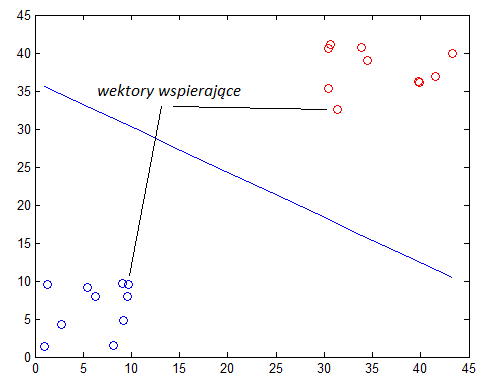
\includegraphics{support_vectors}\\
\caption{Wektory wspierające oznaczone wśród punktów treningowych }
\textit{(opracowanie własne)}
\end{figure}

Klasyfikator maksymalnego marginesu jest klasyfikatorem liniowym i może być użyty do klasyfikacji danych, które są liniowo separowalne. W niniejszym projekcie przyjęto założenie, że separowane dane należą do dwóch klas. Klasyfikator maksymalnego marginesu jest klasyfikatorem binarnym.
Załóżmy teraz, że mamy zbiór danych uczących składających się z $n$ punktów postaci:
\newpage
\begin{equation}
 (\overrightarrow{x_1}, y_1),(\overrightarrow{x_2}, y_2),...,(\overrightarrow{x_n}, y_n)
\end{equation}

\vspace{5mm}
gdzie $y_i$ to 1 lub -1 w zależności od klasy, do której należą, czyli od położenia po dodatniej lub ujemnej stronie hiperpłaszczyzny $H$. Każdy wektor $\overrightarrow{x_i}$ jest rozmiaru $p$. Działanie algorytmu SVM polega na znalezieniu hiperpłaszczyzny  o maksymalnym marginesie geometrycznym, która dzieli grupy punktów $\overrightarrow{x_i}$, dla których $y_i$ = -1 od grupy punktów  $\overrightarrow{x_i}$, dla których $y_i$ = 1.
Hiperpłaszczyzna $H$, $n$-wymiarowa określona jest wzorem:

\vspace{5mm}
\begin{equation}
(H)y(\overrightarrow{x}) = 0
\end{equation}

\vspace{5mm}
gdzie $(y(\overrightarrow{x}) = w^t + b$, $w$ - wektor wagowy, $b$ - wyraz wolny. 
Po przedstawionym wcześniej założeniu, że $y(x)$ = -1 lub $y(x)$ = 1, możemy przedstawić wzór na odległość punktu $x$ od danej hiperpłaszczyzny $H$. Przedstawia się on następująco:

\vspace{5mm}
\begin{equation}
d(x,H) = \frac{|y(x)|}{||w||}
\end{equation}

\vspace{5mm}margines geometryczny natomiast, będzie dany wzorem:

\vspace{5mm}
\begin{equation}
\gamma = \frac{1}{||w||}
\end{equation}

\vspace{5mm}Klasyfikator maksymalnego marginesu znajduje hiperpłaszczyznę, która maksymalizuje wartość marginesu geometrycznego czyli taką, dla której wartość  $||w||$ jest minimalna. 
Maksymalizacja marginesu może zostać zapisana w postaci poniżej przedstawionego problemu optymalizacyjnego:

\vspace{5mm}\centerline {$minimalizacja$  $||\overrightarrow{w}||^2$}

\vspace{5mm} przy warunkach:

\vspace{5mm}\centerline {$y_i(\overrightarrow{w}*\overrightarrow{x_i} - b)\geq 1$}

\vspace{5mm}gdzie $i \in \{1..N\}$ oraz istnieje założenie o liniowej separowalności wektorów.

\vspace{5mm}Można następnie dla powyższego problemu optymalizacyjnego zapisać lagranżjan postaci:

\vspace{5mm}
\begin{equation}
L(w,b,\overrightarrow{\alpha}) = \frac{1}{2}\cdot||\overrightarrow{w}||^2 - \sum_{i=1}^{\ N} \alpha_i(y_i(\overrightarrow{w}* \overrightarrow{x_i} +b)-1) 
\end{equation} 

\vspace{5mm} gdzie $\overrightarrow{\alpha}$ to wektor mnożników Lagrange'a, o rozmiarze $N$.

\vspace{5mm} Korzystając z lagranżjanu, przedstawiony problem optymalizacyjny może zostać zamieniony na formę dualną, w której funkcja celu jest wyłącznie zależna od mnożników Lagrange'a:

\vspace{5mm}\centerline {$minimalizacja$  $funkcji:$}

\vspace{5mm}\centerline {$\frac{1}{2} \sum_{i=1}^{\ N} \sum_{j=1}^{\ N} y_i y_j (\overrightarrow{x_i}\cdot\overrightarrow{x_j}) \alpha_i \alpha_j - \sum_{i=1}^{\ N} \alpha_i$}
  
\vspace{5mm} gdzie $N$ to liczba punktów treningowych

\vspace{5mm} przy warunkach:

\vspace{5mm}\centerline {$\alpha_i \geq 0, \forall i$ }

\vspace{5mm}\centerline {$\sum_{i=1}^{\ N} y_i \alpha_i$ = 0 }

\vspace{5mm}

Kiedy współczynniki Lagrange'a zostaną wyznaczone, wektor $\overrightarrow{w}$ oraz wyraz wolny $b$ może zostać obliczony przy ich pomocy:
\begin{equation}
\overrightarrow{w} = \sum_{i=1}^{\ N} y_i \alpha_i \overrightarrow{x}_i,  
\end{equation}

\begin{equation}
b = \overrightarrow{w} \cdot \overrightarrow{x}_i - y_i  
\end{equation}
dla pewnych  $\alpha_i > 0 $

\vspace{5mm}Oczywiście, nie wszystkie zbiory danych mogą być liniowo separowalne. Może się okazać, że nie istnieje hiperpłaszczyzna, które rozdziela wszystkie punkty należące do jednej klasy od punktów należących do drugiej klasy. W takim właśnie przypadku można skorzystać z pewnej modyfikacji oryginalnego problemu optymalizacyjnego. Prezentuje się ona następująco: 

\vspace{5mm}\centerline {$minimalizacja$  $||\overrightarrow{w}||^2+ C \sum_{i=1}^{\ N} \xi_i$}

\vspace{5mm} przy warunkach:

\vspace{5mm}\centerline {$y_i(\overrightarrow{w} \cdot \overrightarrow{x_i} - b)\geq 1 - \xi_i, \forall_i$}

\vspace{5mm}gdzie $\xi_i$ to tak zwana zmienna luzu, która pozwala na błąd marginesu. 

\vspace{5mm} Klasyfikator w tym wypadku bierze pod uwagę możliwe wahania wartości danych. Wektory wspierające w tym wypadku to nie tylko punkty znajdujące się najbliżej hiperpłaszczyzny, ale również dalsze. 

\vspace{5mm}Forma dualna powyższego problemu przedstawia się następująco:

\vspace{5mm}\centerline {$minimalizacja$  $funkcji:$}

\vspace{5mm}\centerline {$\frac{1}{2} \sum_{i=1}^{\ N} \sum_{j=1}^{\ N} y_i y_j  K(\overrightarrow{x_i} \cdot\overrightarrow{x_j}) \alpha_i \alpha_j - \sum_{i=1}^{\ N} \alpha_i$}
  
\vspace{5mm} gdzie $N$ to liczba punktów treningowych

\vspace{5mm} przy warunkach:

\vspace{5mm}\centerline {$0 \leq \alpha_i \leq C, \forall i$ }

\vspace{5mm}\centerline {$\sum_{i=1}^{\ N} y_i \alpha_i$ = 0 }

\vspace{5mm} W tym wypadku współczynniki $\alpha$ będą również ograniczone z góry. 

\vspace{5mm} Powyższy problem optymalizacyjny może zostać rozwiązany przy pomocy algorytmu \textit{sekwencyjnej minimalnej optymalizacji} który został szczegółowo opisany w kolejnym podrozdziale. 

\newpage
\subsubsection{Sekwencyjna minimalna optymalizacja (SMO)}
SMO jest jednym z algorytmów pozwalających rozwiązać główny problem w nauczaniu SVM, czyli problem programowania kwadratowego (oznaczany jako \textit{QP}). SMO pozwala na uniknięcie problemów związanych z optymizacją numeryczną poprzez rozkład  całościowego problemu na podproblemy.


W każdym kroku SMO rozwiązuje najmniejszy możliwy problem optymalizacji, czyli przypadek dwóch współczynników Lagrange'a, które są ograniczone liniowo. Oba współczynniki są jednocześnie optymalizowane, po czym aktualizowana jest cała maszyna wektorów nośnych i następnie algorytm wybiera dwa kolejne współczynniki do optymalizacji.


SMO jest proste w implementacji oraz nie wymaga dużych zasobów pamięci do przechowywania zmiennych.


SMO składa się z dwóch części - analitycznego poszukiwania pary współczynników Lagrange'a oraz heurystyki służącej wybieraniu kolejnych współczynników do optymalizacji.

\subsubsection{Poszukiwanie współczynników Lagrange'a}

Pierwszą czynnością, którą realizuje SMO, jest obliczenie ograniczeń współczynników. Po ich obliczeniu możliwa jest poszukiwanie minimum w ograniczonej przestrzeni. 

Liniowy warunek równości powoduje, że współczynniki Lagrange'a leżą na prostej, przez co minimum optymalizowanej funkcji również musi na niej leżeć.
Aby SMO spełniało ten warunek w każdym kroku, konieczne jest użycie dwóch współczynników.

Algorytm oblicza drugi współczynnik  Lagrange'a $\alpha_{2}$, po czym oblicza końce odcinka leżącego na prostej spełniającej warunek równości. Jeżeli koniec $y_1$ nie jest równy końcowi $y_2$, wtedy stosuje się następujące ograniczenia dla $\alpha_2$:

\begin{equation}
L = max(0,\alpha_2 - \alpha_1),\quad H = (C,C + \alpha_2 - \alpha_1)
\end{equation}

Jeżeli koniec $y_1$ jest równy końcowi $y_2$, wtedy ograniczenia $\alpha_2$ zmieniają się następująco:

\begin{equation}
L = max(0,\alpha_2 + \alpha_1 - C),\quad H = (C, \alpha_2 + \alpha_1)
\end{equation}

Drugą pochodną funkcji docelowej wzdłuż odcinka można wyrazić jako:

\begin{equation}
\eta = K(\overrightarrow{x_1},\overrightarrow{x_1}) + K(\overrightarrow{x_2},\overrightarrow{x_2}) - 2K(\overrightarrow{x_1},\overrightarrow{x_2})
\end{equation}

W normalnych warunkach funkcja docelowa będzie określona dodatnio, minimum wystąpi wzdłuż prostej określonej liniowym warunkiem równości i $\eta$ będzie większe od zera. W takim przypadku SMO oblicza nieograniczone minimum wzdłuż całej prostej zgodnie z równaniem:

\begin{equation}
\label{alfa2nowy}
\alpha_2^nowy = \alpha_2 + \frac{y_2(E_1-E_2)}{\eta},
\end{equation}

w którym $E_i = u_i - y_i$ oznacza błąd $i$-tej próbki ze zbioru uczącego. W kolejnym kroku znajdywane jest ograniczenie minimum poprzez porównanie z obliczonymi wcześniej końcami odcinka.

\begin{equation}
\alpha_2^{nowy,ograniczony} =  \begin{cases} 
H & \text{jeżeli} \qquad \alpha_2^{nowy} \geq H \\
\alpha_2^{nowy} & \text{jeżeli} \qquad L < \alpha_2^{nowy} < H \\
L & \text{jeżeli} \qquad \alpha_2^{nowy} \leq L
\end{cases}
\end{equation}

Używając oznaczenia $s=y_1 y_2$ wartość $\alpha_1$ można obliczyć wykorzystując nowy, ograniczony współczynnik $\alpha2$:

\begin{equation}
\alpha_1^{nowy} = \alpha_1 + s(\alpha_2 - \alpha_2^{nowy, ograniczony)}).
\end{equation}

W niezwykłych przypadkach $\eta$ nie będzie dodatnie. Ujemne $\eta$ wystąpi, gdy jądro $K$ nie spełni warunku Mercera, przez co funkcja docelowa może stać się nieoznaczona. Zerowe $\eta$ może wystąpić nawet z poprawnym jądrem, gdy więcej niż jedna próbka ucząca ma taki sami wektor wejściowy $x$. SMO zadziała nawet gdy $\eta$ nie jest dodatnie, w takim przypadku funkcja docelowa $\Psi$ powinna zostać policzona na każdym z końców odcinka:


\begin{equation}
f_1 = y_1(E_1+b) - \alpha_1 
\end{equation}
\begin{equation}
f_2 = y_2(E_2+b) - s\alpha_1
\end{equation}
\begin{equation}
K(\overrightarrow{x_1}, \overrightarrow{x_2}) - \alpha_2 K(\overrightarrow{x_2},\overrightarrow{x_2}),
\end{equation}
\begin{equation}
L_1 = \alpha_1 + s(\alpha_2 - L),
\end{equation}
\begin{equation}
H_1 = \alpha_1 + s(\alpha_2 - H),
\end{equation}
\begin{equation}
\Psi_L = L_1 f_1 + Lf_2 + \frac{1}{2}L_1^2 K(\overrightarrow{x_1},\overrightarrow{x_1}) + \frac{1}{2}L^2 K(\overrightarrow{x_2},\overrightarrow{x_2}) + sLL_1 K(\overrightarrow{x_1},\overrightarrow{x_2}), 
\end{equation}
\begin{equation}
\Psi_H = H_1 f_1 + Hf_2 + \frac{1}{2}H_1^2 K(\overrightarrow{x_1},\overrightarrow{x_1}) + \frac{1}{2}H^2 K(\overrightarrow{x_2},\overrightarrow{x_2}) + sHH_1 K(\overrightarrow{x_1},\overrightarrow{x_2}).
\end{equation}


SMO przesunie współczynniki Lagrange'a na ten koniec odcinka, w którym wartość funkcji docelowej jest najmniejsza. Jeżeli funkcja docelowa ma takie same wartości na obu końcach odcinka (uwzględniając mały błąd $\epsilon$ z powodu błędów zaokrągleń) i jądro spełnia warunki Mercera, to optymalizacja nie może się zakończyć. Ten przypadek opisano poniżej.

\subsubsection{Heurystyka wyboru współczynników do optymalizacji}


Wartość funkcji docelowej zmniejszy się w każdym kroku działania algorytmu SMO, jeżeli zostanie zoptymalizowana para współczynników Lagrange'a i co najmniej jeden z nich przed optymalizacją łamał warunki KKT. To gwarantuje zbieżność algorytmu, której uzyskanie można przyspieszyć stosując heurystykę do wyboru pary współczynników do jednoczesnej optymalizacji.


Stosowane do tego są dwie różne heurystyki wyboru współczynników. Wybór pierwszego współczynnika gwarantuje zewnętrzna pętla algorytmu - iteruje po całym zbiorze uczącym sprawdzając które z przypadków naruszają warunki KKT. Jeżeli dana próbka nie spełnia tych warunków, może być optymalizowana. Po przejściu przez cały zbiór uczący, zewnętrzna pętla ponownie iteruje po wszystkich próbkach, dla których współczynniki Lagrange'a są różne od 0 i różne od $C$ (przypadki niegraniczne). Ponownie dla każdego z takich przypadków są sprawdzane warunki KKT i optymalizacji mogą podlegać te, które ich nie spełniają. Zewnętrzna pętla powtarza przejścia po wszystkich przypadkach niegranicznych dopóki wszystkie przypadki naruszające warunki KKT nie będą leżały w granicach błędu $\epsilon$. Następnie zewnętrzna pętla cofa się i ponownie iteruje po całym zbiorze uczącym. Pętla ta przełącza się między pojedynczymi przejściami po całym zbiorze uczącym i wielokrotnymi przejściami po podzbiorze niegranicznym do momentu, w którym cały zbiór spełnia warunki KKT w granicach $\epsilon$. W tym momencie algorytm kończy działanie.


Heurystyka pierwszego wyboru skupia się na przypadkach, dla których prawdopodobieństwo złamania warunków KKT jest największe, czyli dla zbioru niegranicznego. Przypadki, które znajdują się na granicy, najprawdopodobniej na niej pozostaną, a te, które nie są na granicy, mogą się przesunąć. SMO optymalizuje więc najpierw podzbiór danych, a następnie przeszukuje cały zbiór w poszukiwaniu punktów, które mogły zacząć łamać warunki KKT w wyniki wcześniejszych zmian.


Typowa wartość błędu $\epsilon$, dla którego warunki KKT są spełnione, to $10^{-3}$. Zmniejszenie wartości dopuszczalnego błędu może spowodować wydłużenie czasu potrzebnego na optymalizację, jednak jest to typowe dla wszystkich algorytmów stosowanych do nauki SVM.


Po wyborze pierwszego współczynnika Lagrange'a, wybierany jest drugi współczynnik w taki sposób, aby zmaksymalizować wielkość kroku podczas optymalizacji pary. Obliczanie funkcji jądra $K$ jest czasochłonne, więc SMO przybliża wielkość kroku o wartość bezwzględną licznika w równaniu \ref{alfa2nowy}: $|E_1 - E_2|$. SMO zapisuje wartość błędu $E$ dla każdego przypadku niegranicznego w zbiorze uczącym i wybiera błąd tak, aby zmaksymalizować wielkość kroku. Jeżeli $E_1$ jest dodatnie, SMO wybierze przypadek z najmniejszą wartością błędu $E_2$. Jeżeli $E_1$ jest ujemne, SMO wybierze przypadek z największym błędem $E_2$.


W wyjątkowych sytuacjach SMO nie może znaleźć odpowiedniego współczynnika przy wykorzystaniu opisanej heurystyki drugiego wyboru, np. w przypadku, gdy dwie próbki mają takie same wartości cech. W takim przypadku SMO stosuje hierarchię heurystyki drugiego wyboru aż znajdzie parę współczynników Lagrange'a, które mogą być optymalizowane. Warunkiem skutecznej optymalizacji jest wykonanie niezerowego kroku. Hierarchię w tym przypadku można przestawić następująco - jeżeli optymalizacja nie jest skuteczna, SMO iteruje po przypadkach niegranicznych, poszukując przypadku, który pozwoli na sukces. Jeżeli żaden z niegranicznych przypadków na to nie pozwala, SMO zaczyna iterować po całym zbiorze uczącym aż zostanie znaleziony przypadek pozwalający na skuteczną optymalizację. Iterowanie zarówno w przypadku podzbioru przypadków niegranicznych jak i całego zbioru rozpoczyna się od losowo wybranego elementu zbioru. Pozwala to uniknąć obciążenia SMO przez elementy znajdujące się na początku zbioru. W najgorszym przypadku żaden z pozostałych przypadków nie będzie się nadawał do optymalizacji. W takiej sytuacji dana próbka jest pomijana i SMO przechodzi do kolejnej wybranej próbki.


\subsubsection{Obliczanie progu}


Próg $b$ jest obliczany w każdym kroku, dzięki czemu warunki KKT są spełnione dla obu optymalizowanych próbek. Przedstawiony na równaniu próg $b_1$ jest prawidłowy, gdy nowy współczynnik $\alpha_1$ nie jest na granicy, ponieważ zmusza SVM, aby wyjściem było $y_1$ dla wejścia $x_1$:

\begin{equation}
b_1 = E_1 + y_1(\alpha^{nowy}_1 - \alpha_1)K(\overrightarrow{x_1},\overrightarrow{x_1}) + y_2(\alpha^{nowy}_2 - \alpha_2)K(\overrightarrow{x_1},\overrightarrow{x_2}) + b
\end{equation}


Opisany poniżej próg $b_2$ jest prawidłowy, gdy nowy współczynnik $\alpha_2$ nie leży na granicy, ponieważ zmusza SVM, aby wyjściem było $y_2$ dla wejścia $x_2$:

\begin{equation}
b_2 = E_2 + y_1(\alpha^{nowy}_1 - \alpha_1)K(\overrightarrow{x_1},\overrightarrow{x_2}) + y_2(\alpha^{nowy}_2 - \alpha_2)K(\overrightarrow{x_2},\overrightarrow{x_2}) + b
\end{equation}

Jeżeli oba progi $b_1$ i $b_2$ są prawidłowe, to są sobie równe. Gdy oba współczynniki Lagrange'a leżą na granicy i gdy $L$ nie jest równe $H$, wtedy odległością między $b_1$ i $b_2$ są wszystkie progi, które są zgodne z warunkami KKT. SMO wybiera wtedy próg leżący pośrodku między $b_1$ oraz $b_2$.

\subsection{Opis sposobu implementacji algorytmu}

\subsubsection{Schematy blokowe działania algorytmu}

Sposób działania algorytmu przedstawiono za pomocą trzech schematów blokowych, które znajdują się poniżej:

\begin{center}
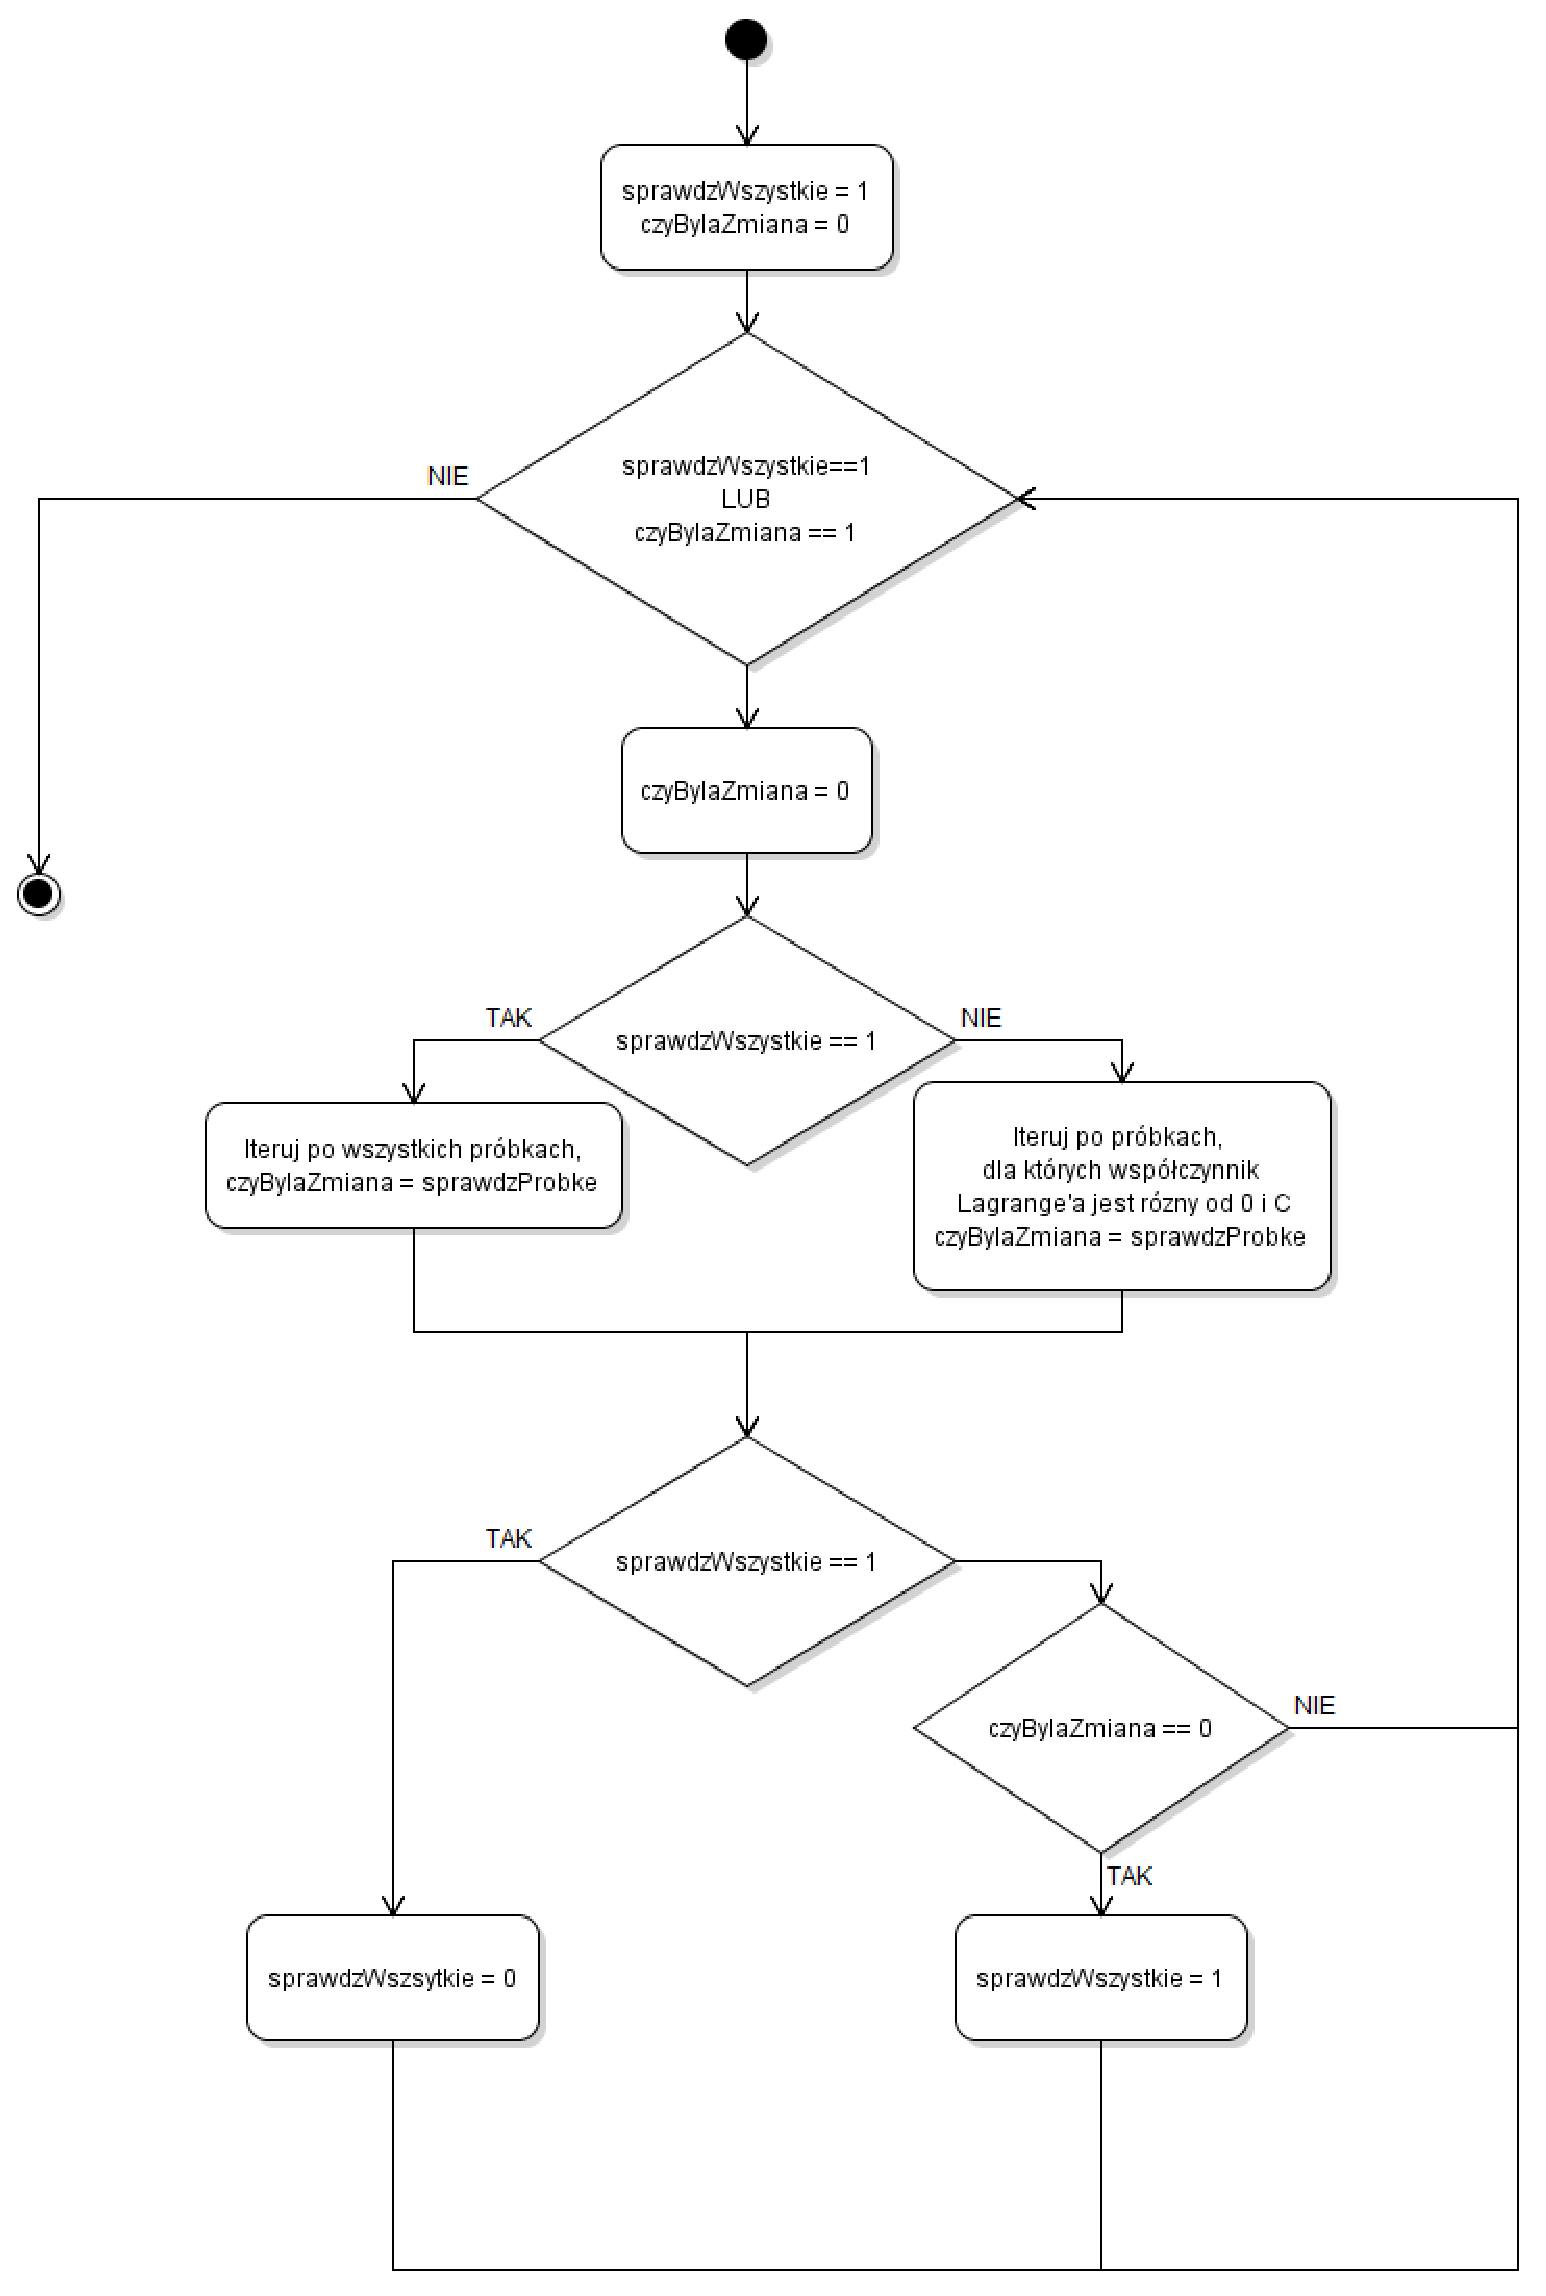
\includegraphics[scale=0.6]{mainloop}\\
\captionof{figure}{ Schemat blokowy głównej pętli programu }
\textit{(opracowanie własne)}
\end{center}

\begin{center}
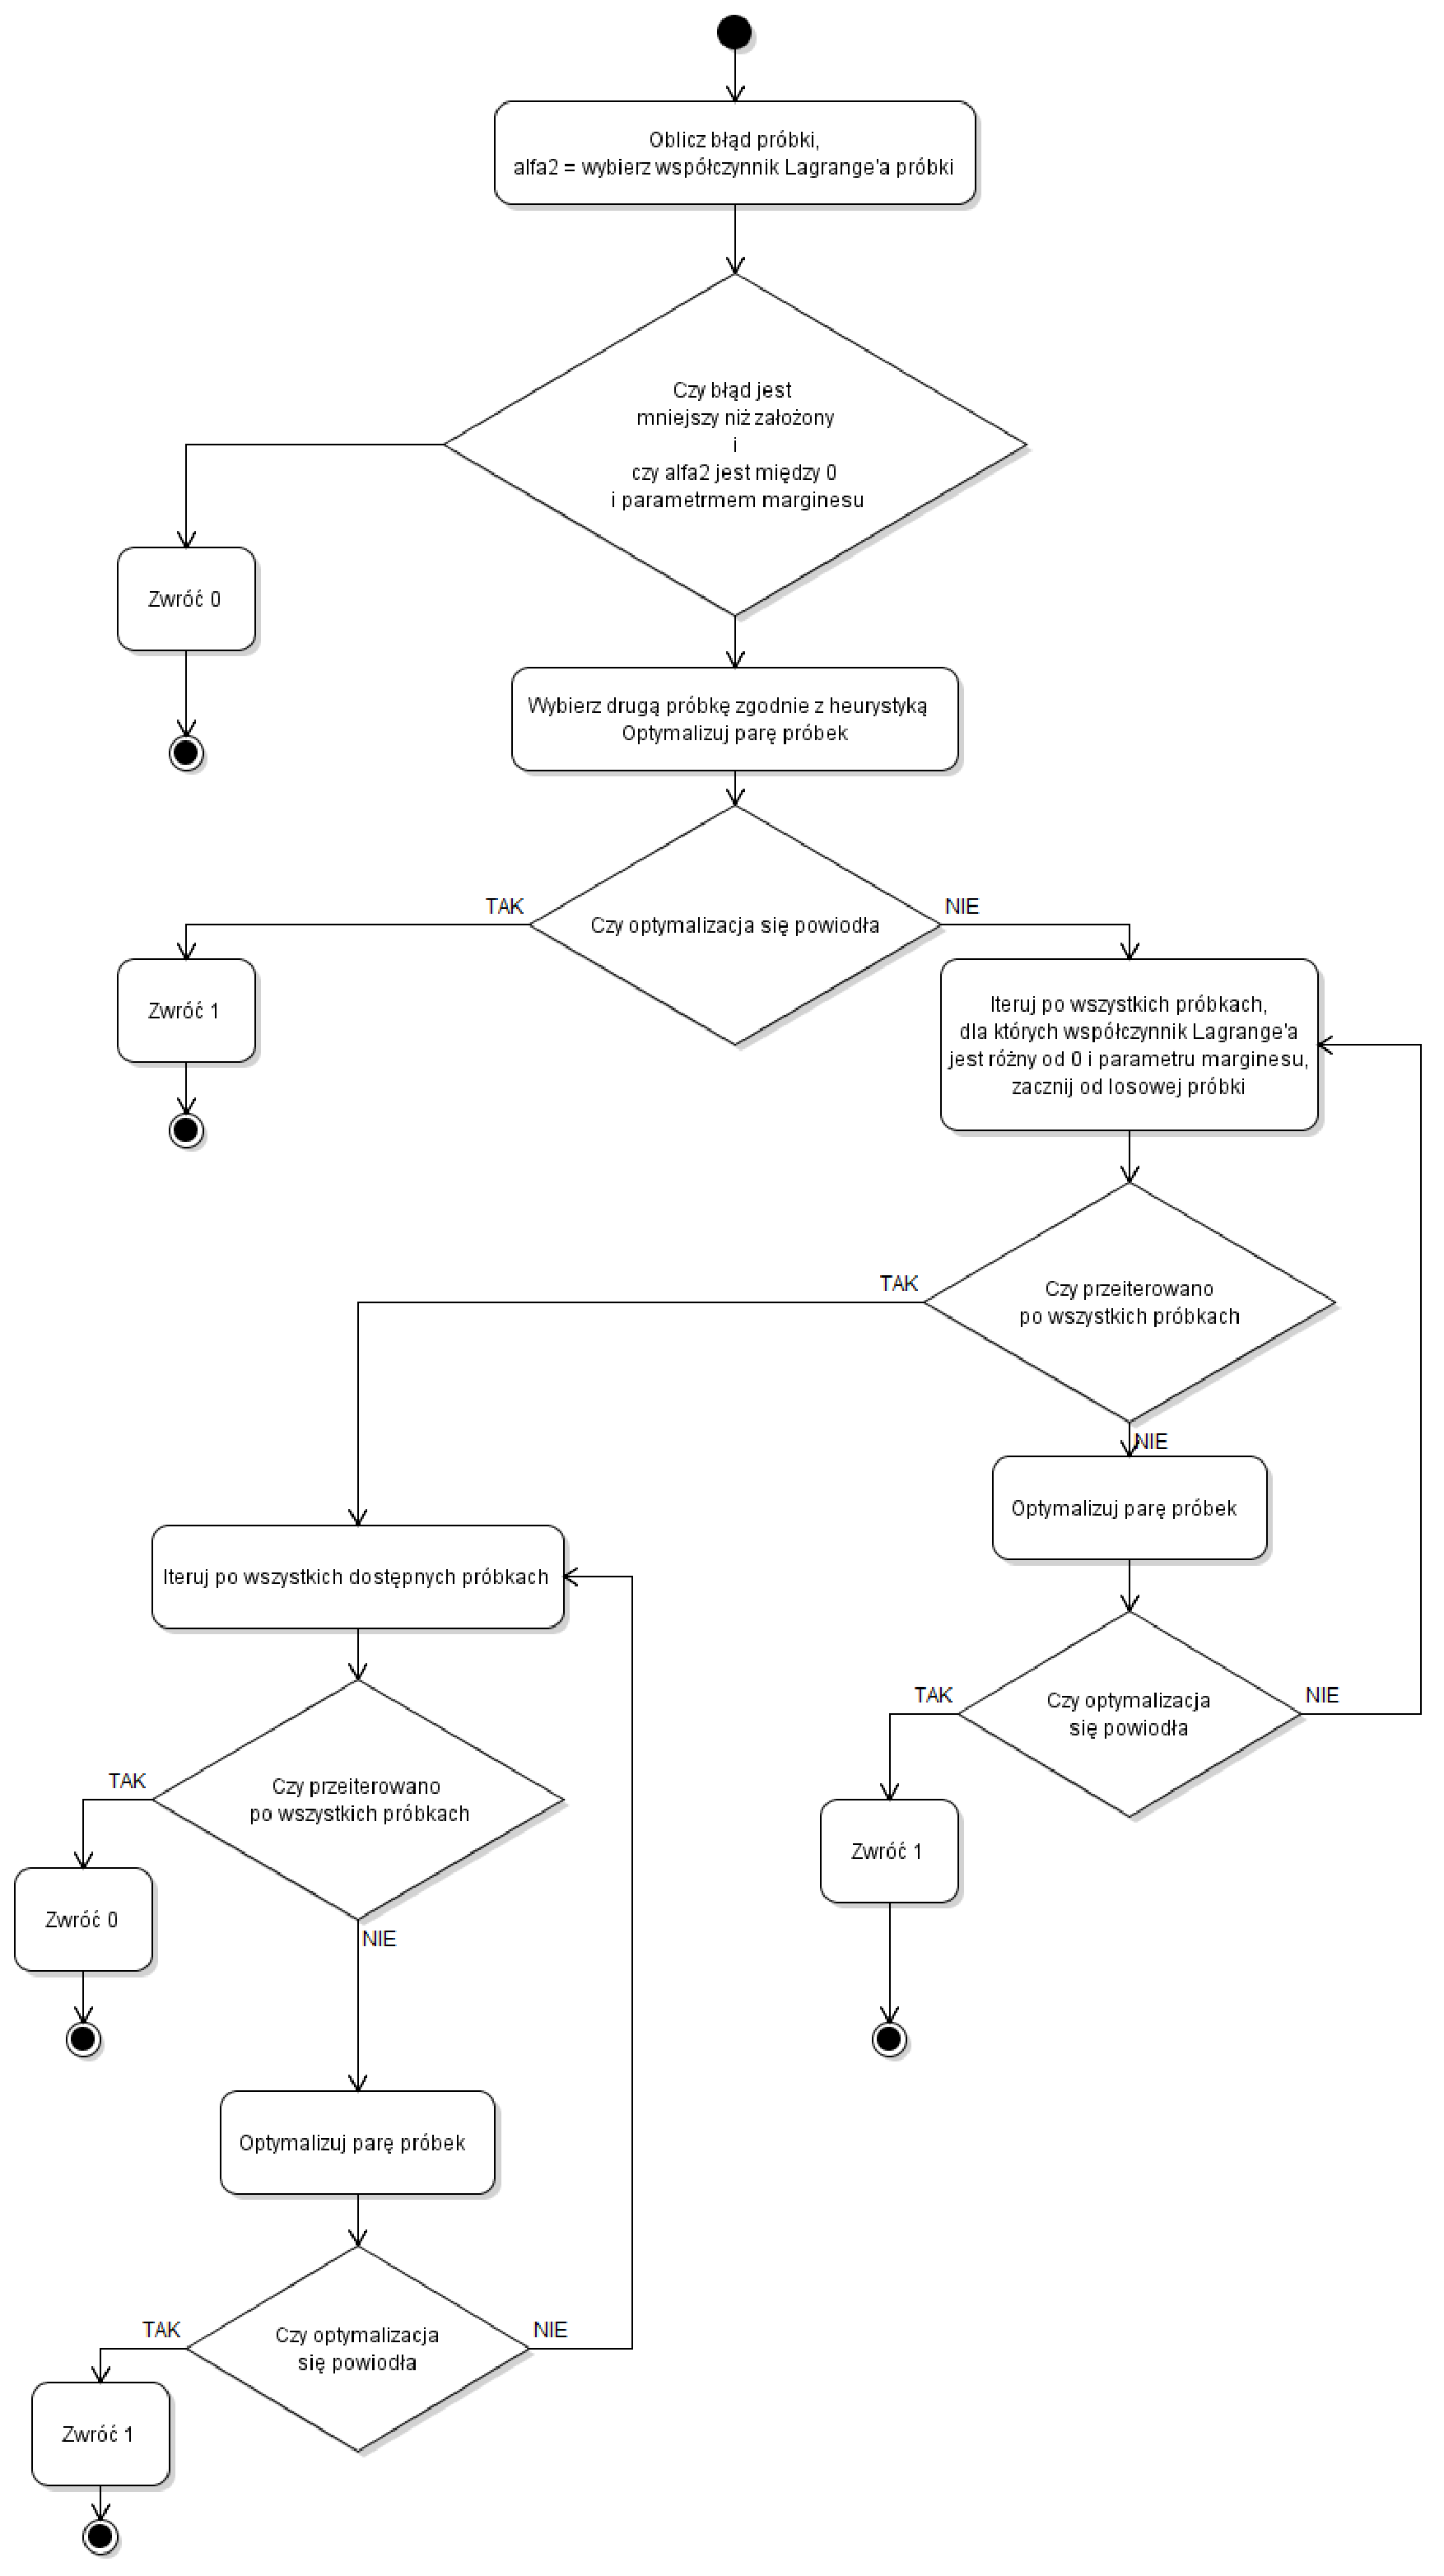
\includegraphics[scale=0.45]{examineExample}\\
\captionof{figure}{ Schemat blokowy badania pojedynczej obserwacji }
\textit{(opracowanie własne)}
\end{center}

\begin{center}
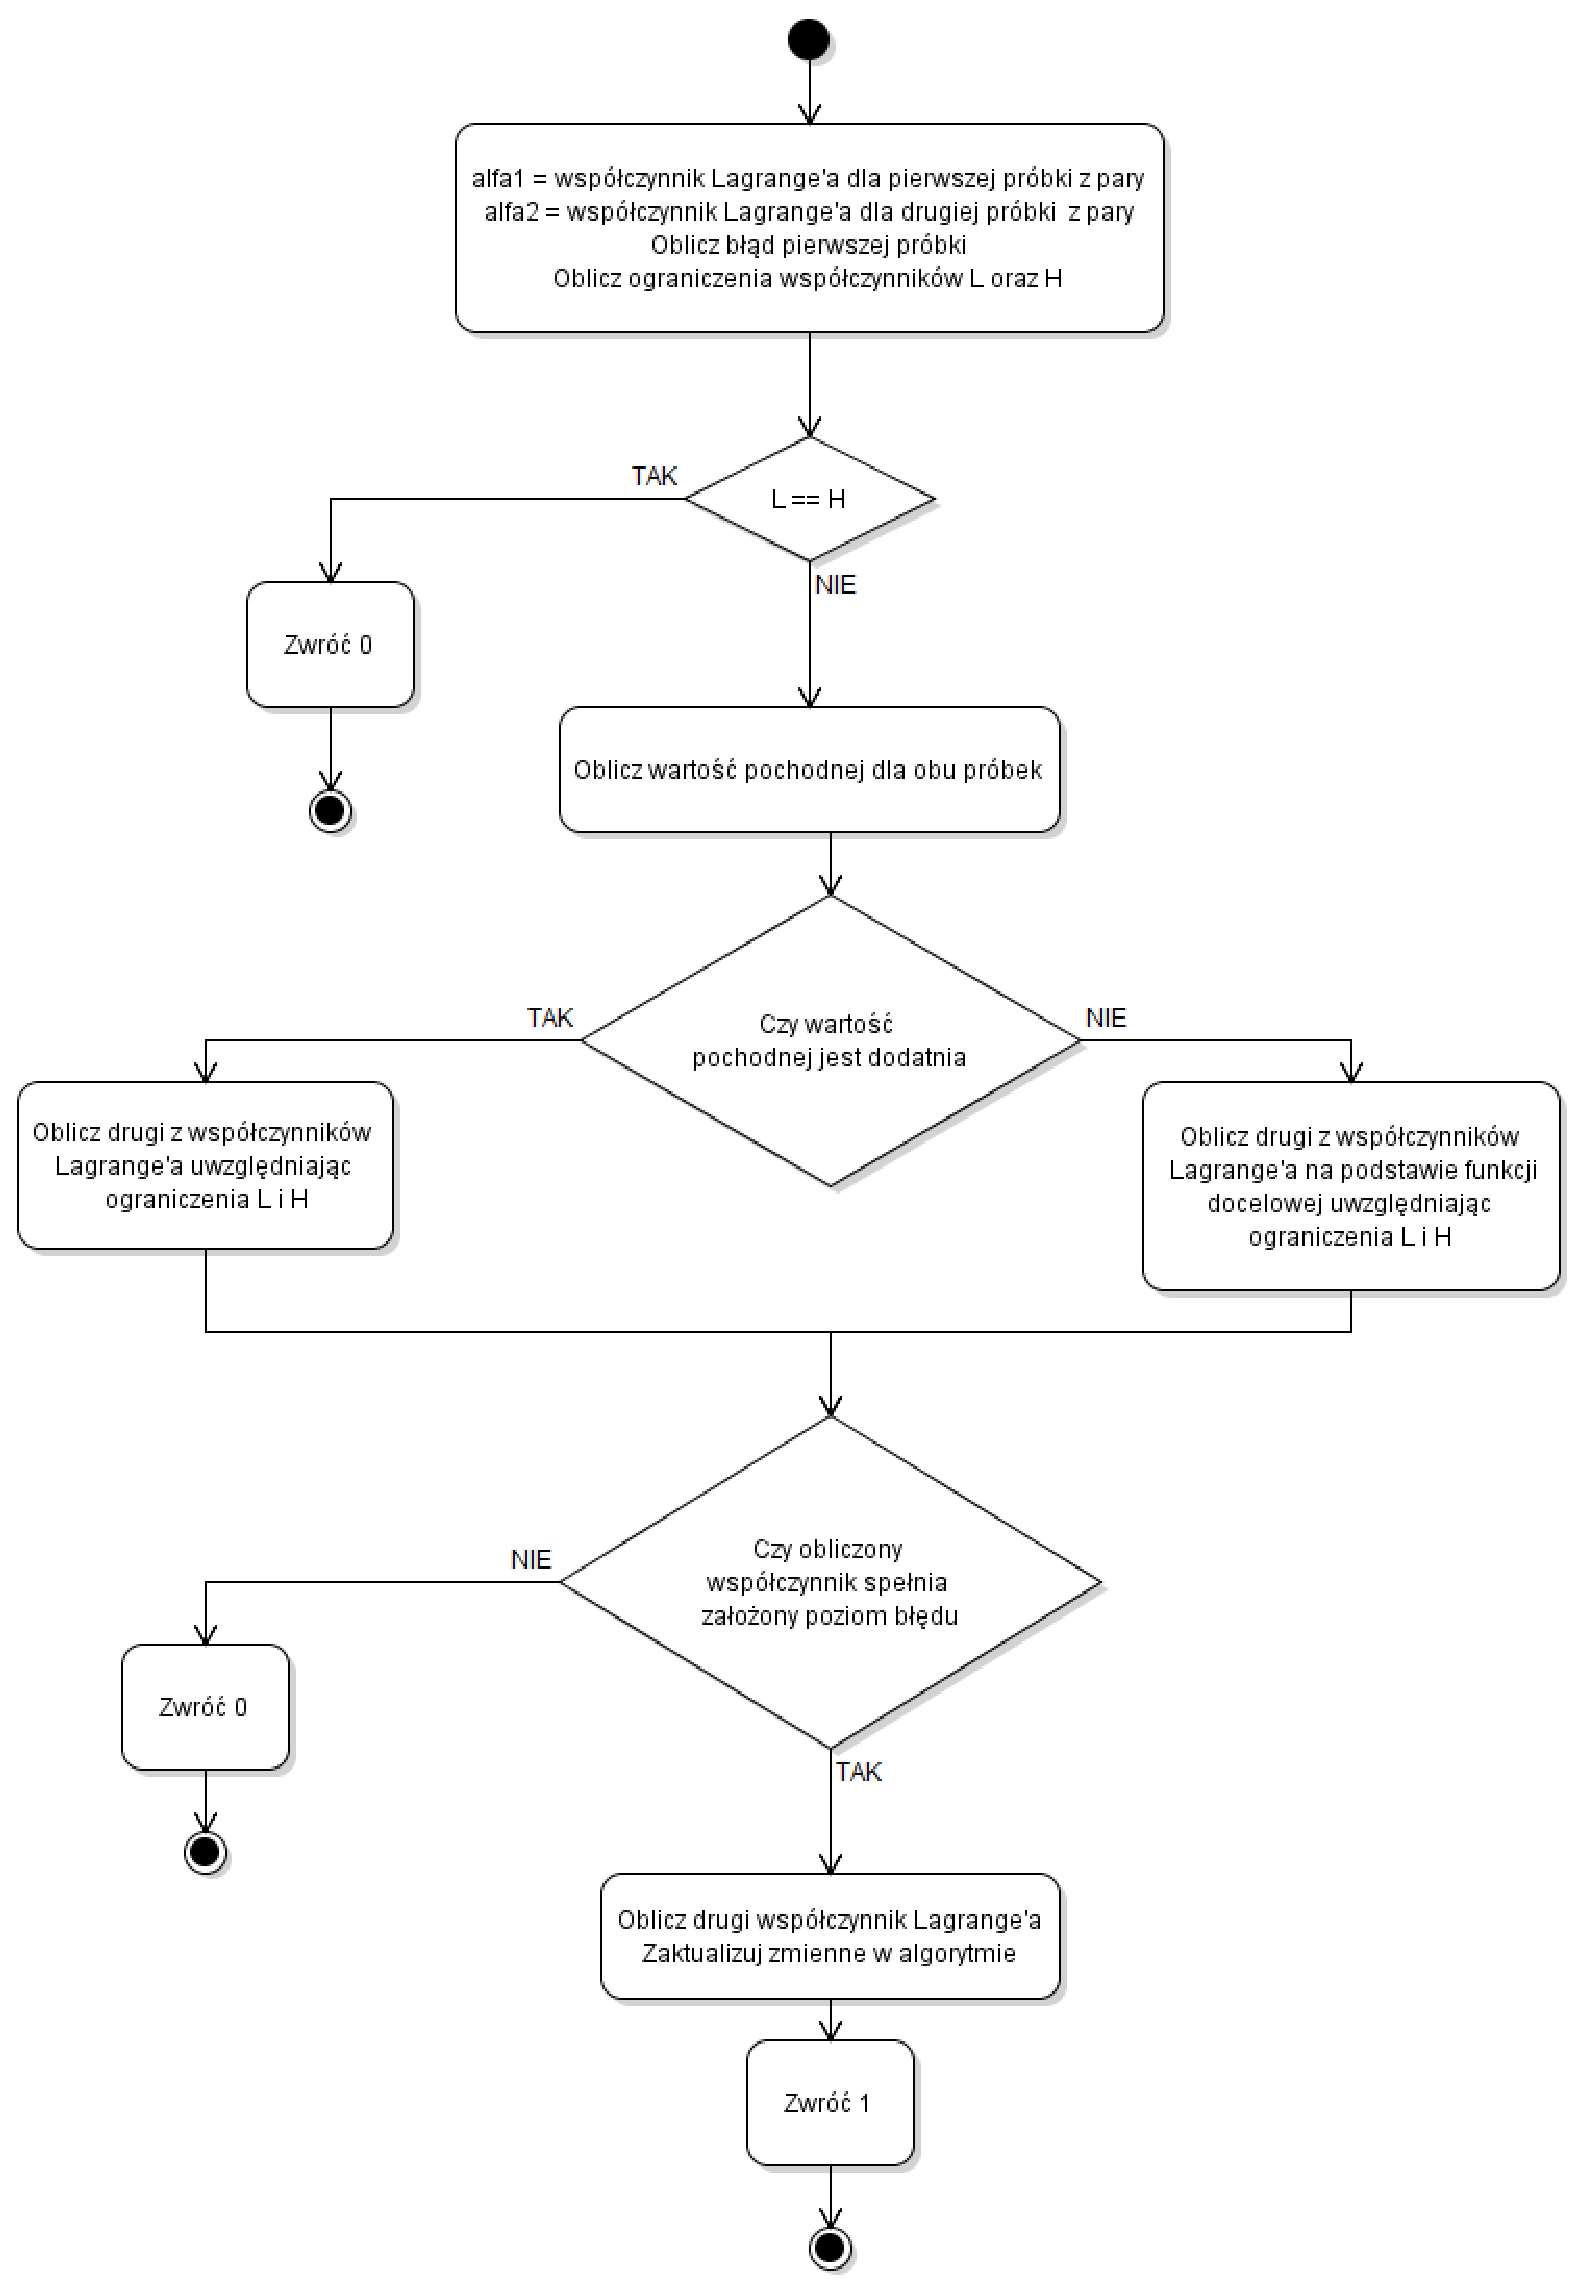
\includegraphics[scale=0.6]{optimizePair}\\
\captionof{figure}{ Schemat blokowy optymalizacji pary próbek }
\textit{(opracowanie własne)}
\end{center}

\subsection{Wizualizacja działania algorytmu}
W celu zobrazowania sposobu działania prototypu algorytmu opracowanego w środowisku MATLAB, dokonano wizualizacji wyznaczonej hiperpłaszczyzny. Dane należące do dwóch różnych kategorii zostały wylosowane przy pomocy funkcji $rand()$.
\subsubsection{Wizualizacja dla dwóch cech}
Na rysunku nr 4 przedstawiono dwa zbiory punktów należących do dwóch różnych klas, które zostały rozdzielone przy pomocy obliczonej hiperpłaszczyzny. W tym wypadku użyto dwóch cech, a przedstawione dane były liniowo separowalne. 
\begin{figure}[h]
\centering
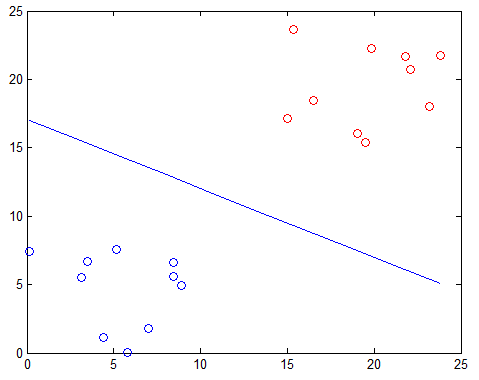
\includegraphics{visualize1}\\
\caption{Rezultat działania algorytmu dla dwóch wymiarów cech i liniowo separowalnych danych }
\textit{(opracowanie własne)}
\end{figure}

\newpage
Na rysunku nr 5 przedstawiono dwa zbiory punktów należących do dwóch różnych klas, które zostały rozdzielone przy pomocy obliczonej hiperpłaszczyzny. W tym wypadku użyto dwóch cech, a przedstawione dane nie były liniowo separowalne. 
\begin{figure}[h]
\centering
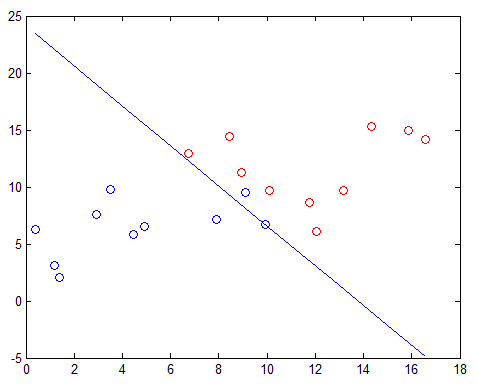
\includegraphics{visualize2}\\
\caption{Rezultat działania algorytmu dla dwóch wymiarów cech i danych nieseperowalnych liniowo  }
\textit{(opracowanie własne)}
\end{figure}

\subsubsection{Wizualizacja dla trzech cech}
Na rysunku nr 6 przedstawiono dwa zbiory punktów należących do dwóch różnych klas, które zostały rozdzielone przy pomocy obliczonej hiperpłaszczyzny. W tym wypadku użyto trzech cech, a przedstawione dane  były liniowo separowalne. 

\begin{figure}[h]
\centering
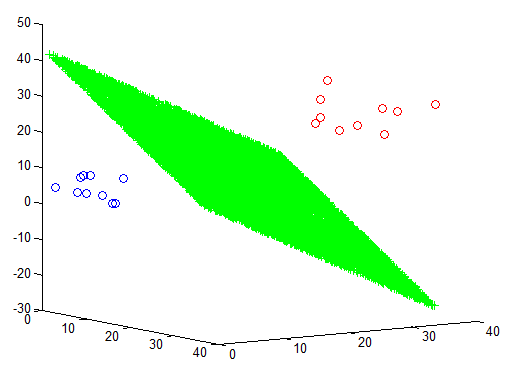
\includegraphics{visualize3}\\
\caption{Rezultat działania algorytmu dla trzech wymiarów cech i liniowo separowalnych danych }
\textit{(opracowanie własne)}
\end{figure}

Na rysunku nr 7 przedstawiono dwa zbiory punktów należących do dwóch różnych klas, które zostały rozdzielone przy pomocy obliczonej hiperpłaszczyzny. W tym wypadku użyto trzech cech, a przedstawione dane nie były liniowo separowalne. 

\begin{figure}[h]
\centering
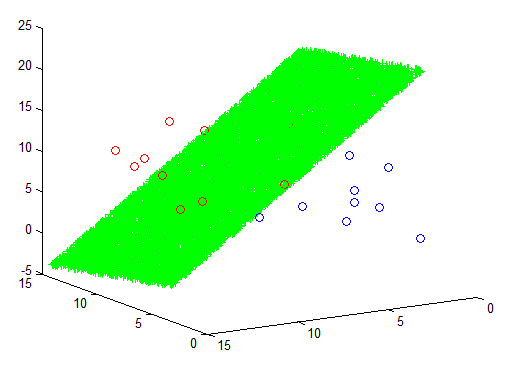
\includegraphics{visualize4}\\
\caption{Rezultat działania algorytmu dla trzech wymiarów cech i danych nieseperowalnych liniowo }
\textit{(opracowanie własne)}
\end{figure}


\subsection{Opis informatyczny procedur}


\fbox{funkcja optimizePair:}\\
\newline
\textbf {void optimizePair(MatrixXd labelSet, MatrixXd gramMatrix, int pairFirst, int pairSecond, MatrixXd sampleError, MatrixXd \&lagrangeMultipliers, double const marginParameter, double \&bias, bool \&flagOptimizeSuccess)}\\
\newline
\vspace{3mm}Funkcja pozwala na optymalizację pary współczynników Lagrange'a.\\
\vspace{3mm}Funkcja przyjmuje:\\
labelSet - macierz typu MatrixXd z oznaczeniem cech\\
gramMatrix - macierz typu MatrixXd reprezentującą macierz Gramma\\
pairFirst - liczba typu int reprezentująca analizowany indeks \\
pairSecond - liczba typu int reprezentująca analizowany indeks \\
sampleError macierz typu MatrixXd zawierająca wartości błędu dla poszczególnych próbek\\
marginParameter - parametr marginesu \\
\newline
\vspace{3mm}Funkcja przyjmuje w postaci referencji:\\
lagrangeMultipliers - macierz typu MatrixXd ze współczynnikami Lagrange'a\\
bias - liczba typu double oznaczająca przesunięcie granicy decyzyjności\\
flagOptimizeSuccess - wartość logiczna typu bool reprezentująca powodzenie lub niepowdzenie optymalizacji\\
\newline
\newline
\newline
\fbox{funkcja examineSample:}\\
\newline
\textbf {void examineSample(int pairSecond, MatrixXd \&sampleError, MatrixXd \&lagrangeMultipliers, MatrixXd gramMatrix, MatrixXd labelSet, double \&bias, double const marginParameter, double const tolerance, bool \&flagExamineSuccess)}\\
\newline
\vspace{3mm}Funkcja pozwala na analizę danej próbki.\\
\vspace{3mm}Funkcja przyjmuje:\\
pairSecond - liczba typu int reprezentująca analizowany indeks \\
gramMatrix - macierz typu MatrixXd reprezentującą macierz Gramma\\
labelSet - macierz typu MatrixXd z oznaczeniem cech\\
marginParameter - parametr marginesu \\
tolerance - liczba typu double reprezentująca tolerancję\\
\newline
\vspace{3mm}Funkcja przyjmuje w postaci referencji:\\
sampleError macierz typu MatrixXd zawierająca wartości błędu dla poszczególnych próbek\\
lagrangeMultipliers - macierz typu MatrixXd ze współczynnikami Lagrange'a\\
bias - liczba typu double oznaczająca przesunięcie granicy decyzyjności\\
flagExamineSuccess - wartość logiczna typu bool reprezentująca powodzenie lub niepowdzenie analizy\\
\newline
\newline
\newline
\fbox{funkcja smosvm:}\\
\newline
\textbf {void smosvm(MatrixXd trainSet, MatrixXd labelSet, double const marginParameter, MatrixXd \&w, double \&bias, float \&trainingTime)}\\
\newline
\vspace{3mm}Funkcja pozwala na wyznaczenie optymalnej hiperpłaszczyzny rozdzielającej dwie klasy.\\
\vspace{3mm}Funkcja przyjmuje:\\
trainSet - macierz typu MatrixXd zawierającą cechy do trenowania algorytmu\\
labelSet - macierz typu MatrixXd zawierającą oznaczenia cech\\
marginParameter - parametr marginesu \\
\newline
\vspace{3mm}Funkcja przyjmuje w postaci referencji:\\
w - macierz typu MatrixXd zawierającą współczynniki wyznaczonej hiperpłaszczyzny\\
bias - liczba typu double oznaczająca przesunięcie granicy decyzyjności\\
trainingTime - liczbę typu float reprezentującą czas trenowania\\
\newline
\newline
\newline
\fbox{funkcja loadData:}\\
\newline
\textbf {bool loadData(std::string filename, MatrixXd \&dataSet, MatrixXd \&labelSet)}\\
\newline
\vspace{3mm}Funkcja pozwala na wczytanie danych treningowych oraz danych testowych.\\
\vspace{3mm}Funkcja przyjmuje:\\
filename - string z nazwą pliku\\
\newline
\vspace{3mm}Funkcja przyjmuje w postaci referencji:\\
dataSet - macierz typu MatrixXd z cechami które zostały wczytane\\
labelSet - macierz typu MatrixXd z oznaczeniem cech\\
\newline
\vspace{3mm}Funkcja zwraca wartość logiczną typu bool reprezentującą powodzenie lub niepowodzenie procesu wczytywania pliku:\\
\newline
\newline
\newline
\fbox{funkcja svmclassify:}\\
\newline
\textbf {MatrixXd svmclassify(MatrixXd w, double bias, MatrixXd \&dataSet, float \&classificationTime)}\\
\newline
\vspace{3mm}Funkcja pozwala na klasyfikację zbioru testowego przy użyciu wcześniej obliczonych współczynników klasyfikatora.\\
\newline
\vspace{3mm}Funkcja przyjmuje:\\
w - macierz typu MatrixXd zawierającą współczynniki wyznaczonej hiperpłaszczyzny\\
bias - liczba typu double oznaczająca przesunięcie granicy decyzyjności\\
\newline
\vspace{3mm}Funkcja przyjmuje w postaci referencji:\\
dataSet - macierz typu MatrixXd zawierające dane, które mają zostać sklasyfikowane\\
classificationTime - liczba typu float reprezentująca czas klasyfikacji\\
\newline
\vspace{3mm}Funkcja zwraca macierz typu MatrixXd zawierającą wyniki klasyfikacji uzyskanej przez algorytm:\\
\newline
\newline
\newline
\fbox{funkcja checkAccuracy:}\\
\newline
\textbf {float checkAccuracy(MatrixXd const resultSet, MatrixXd const \&trueResultSet)}\\
\newline
\vspace{3mm}Funkcja pozwala na sprawdzenie skuteczności klasyfikacji algorytmu.\\
\vspace{3mm}Funkcja przyjmuje:\\
resultSet - macierz typu MatrixXd z wynikami klasyfikacji uzyskanymi przez algorytm \\
\newline
\vspace{3mm}Funkcja przyjmuje w postaci referencji:\\
trueResultSet - macierz typu MatrixXd z poprawnymi wynikami klasyfikacji\\
\newline
\vspace{3mm}Funkcja zwraca liczbę typu float reprezentującą skuteczność klasyfikacji algorytmu:\\
\newline
\newline
\newline
\fbox{funkcja saveResult:}\\
\newline
\textbf {void saveResult(float const \&trainingTime, float const \&classificationTime, float const \&accuracy)}\\
\newline
\vspace{3mm}Funkcja pozwala na zapisywanie rezultatów treningu oraz klasyfikacji do pliku tekstowego "linear SVM results.txt".\\
\newline
\vspace{3mm}Funkcja przyjmuje w postaci referencji:\\
trainingTime - czas, którego algorytm potrzebował na nauczenie klasyfikatora \\
classificationTime - czas, którego algorytm potrzebował do klasyfikacji\\
accurancy - skuteczność klasyfikacji algorytmu w \% \\
\newline
\newline
\newline
\fbox{funkcja getBiggerNumber:}\\
\newline
\textbf {double getBiggerNumber(double firstNumber, double secondNumber)}\\
\newline
\vspace{3mm}Funkcja pozwala na znalezienie liczby większej spośród dwóch liczb.\\
\vspace{3mm}Funkcja przyjmuje:\\
firstNumber - liczbę typu double\\
secondNumber - liczbę typu double\\
\newline
\vspace{3mm}Funkcja zwraca większą z dwóch analizowanych liczb:\\
\newline
\newline
\newline
\fbox{funkcja getSmallerNumber:}\\
\newline
\textbf {double getSmallerNumber(double firstNumber, double secondNumber)}\\
\newline
\vspace{3mm}Funkcja pozwala na znalezienie liczby mniejszej spośród dwóch liczb.\\
\vspace{3mm}Funkcja przyjmuje:\\
firstNumber - liczbę typu double\\
secondNumber - liczbę typu double\\
\newline
\vspace{3mm}Funkcja zwraca mniejszą z dwóch analizowanych liczb:\\
\newline
\newline
\newline
\fbox{ getNonboundSubset:}\\
\newline
\textbf {MatrixXd getNonboundSubset(MatrixXd lagrangeMultipliers, double marginParameter)}\\
\newline
\vspace{3mm}Funkcja przyjmuje:\\
lagrangeMultipliers - macierz typu MatrixXd ze współczynnikami Lagrange'a\\
marginParameter - liczba typu double z parametrem marginesu\\
\newline
\vspace{3mm}Funkcja zwraca macierz typu MatrixXd z indeksami elementów macierzy lagrangeMultipliers, których wartość jest różna od 0 lub różna od wartości zmiennej marginParameter\\
\newline
\newline
\newline
\fbox{funkcja randomizeIndexOrder:}\\
\newline
\textbf {void randomizeIndexOrder(MatrixXd dataSet, MatrixXd \&randomizedIndices)}\\
\newline
\vspace{3mm}Funkcja pozwala na losowe ustawienie indeksów.\\
\vspace{3mm}Funkcja przyjmuje:\\
dataSet - macierz typu MatrixXd z indeksami, które mają zostać zrandomizowane\\
\newline
\vspace{3mm}Funkcja przyjmuje w postaci referencji:\\
randomizedIndices - macierz typu MatrixXd z indeksami, które zostały zrandomizowane\\
\newline
\newline
\newline
\fbox{funkcja random\_data\_generator:}\\
\newline
\textbf {void random\_data\_generator(MatrixXd \&trainSet, MatrixXd \&labelSet))}\\
\newline
\vspace{3mm}Funkcja pozwala na wylosowanie danych do testowania działania algorytmu.\\
\vspace{3mm}Funkcja przyjmuje w postaci referencji:\\
trainSet - macierz typu MatrixXd z cechami do trenowania\\
labelSet - macierz typu MatrixXd z oznaczeniem klas\\
\begin{thebibliography}{9}

\bibitem{smomain} 
Platt John
\textit{Sequential Minimal Optimization: A Fast Algorithm for Training Support Vector Machines} 
Microsoft Research, Technical Report MSR-TR-98-14, 1998

\bibitem{ecgsvm} 
de Chazal Philip 
\textit{A Patient-Adapting Heartbeat Classifier Using ECG Morphology and Heartbeat Interval Features},
IEEE Transactions On Biomedical Engineering, Vol. 53, No. 12, 2006

\bibitem{stefanowski}
Stefanowski Jerzy
\textit{Metoda wektorów nośnych - slajdy dodatkowe do wykładu} 
\\\texttt{http://www.cs.put.poznan.pl/jstefanowski/ml/SVM.pdf}
Institute of Computing Sciences, Poznań University of Technology


\bibitem{svmtutorial}
SVM Tutorial
\textit{Understending the math}, 
\\\texttt{http://www.svm-tutorial.com/2014/11/svm-understanding-math-part-2/}

\end{thebibliography}
\newpage
\section{Klasyfikator Bayesa}
\subsection{Opis algorytmu}
Działanie klasyfikatora Bayesa polega na przyporządkowaniu nowego przypadku do wcześniej zdefiniowanej klasy.  Podstawowym założeniem tego klasyfikatora jest niezależność każdej cechy występującej w klasie od reszty cech. Innymi słowy użyty klasyfikator bayesowski jest klasyfikatorem probabilistycznym z założeniem niezależności. Oznacza to, że obecność lub brak danej cechy nie łączy się z występowaniem jakiejkolwiek innej. Omawiany klasyfikator jest statystycznym klasyfikatorem opartym na twierdzeniu Bayesa.

\vspace{0.5cm}
Zakłada się, że dany obiekt $X$ jest reprezentowany przez zbiór cech, którego wartości należą do zbioru $X=(x_{1}, x_{2}, ..., x_{n})$. Reguła Bayesa mówi, że obiekt $X$ należy do klasy $C_{j}$, dla której wartość prawdopodobieństwa $P(C_{i}|X)$ jest największa. $P(C|X)$ to prawdopodobieństwo, że obiekt $X$ należy do klasy $C$. Aby oszacować prawdopodobieństwa a-posterori $P(C|X)$ należy skorzystać z twierdzenia Bayesa, które ma postać:

\begin{equation}
P(C|X) = P(X|C)P(C)/P(X)
\end{equation}

gdzie:

$P(C)$ - prawdopodobieństwo a-priori wystąpienia klasy $C$ (czyli prawdopodobieństwo, że dowolny przykład należy do klasy $C$),

$P(X|C)$ - prawdopodobieństwo a-posteriori, że obiekt $X$ należy do klasy~$C$,

$P(X)$ - prawdopodobieństwo wystąpienia obiektu $X$.

\vspace{0.5cm}
Prawdopodobieństwo $P(X)$ jest dla wszystkich klas takie same, więc tak naprawdę klasa $C_{i}$, dla której wartość $P(C|X)$ jest największa to klasa dla której prawdopodobieństwo $P(X|C_{i})P(C_{i})$ jest największe. 

\vspace{0.5cm}
Wartość $P(C_{i})$ zastępuje się względną częstością klasy $C{i}$ lub można założyć, że wszystkie klasy mają takie same prawdopodobieństwo.
 
 \vspace{0.5cm}
Prawdopodobieństwo $P(X|C_{i}$P(X|Ci) to tak naprawdę iloczyn prawdopodobieństw kolejnych atrybutów:

\begin{equation}
P(X|C_{i}) = \prod_{j=1}^{n}P(x_{j}|C_{i})
\end{equation}

W przypadku wystąpienia ciągłego atrybutu prawdopodobieństwo $P(X_{j}|C_{i})$ należy estymować za pomocą funkcji gęstości prawdopodobieństwa przy założeniu normalnego rozkładu wartości atrybutów:


\begin{equation}
f(x) = \frac{1}{\sigma \sqrt{2\pi}}e^{-\frac{(x - \mu)^{2}}{2\sigma^{2}}}
\end{equation}

gdzie:

$\mu$ - średnia danego atrybutu w klasie,

$\sigma^{2}$ - wariancja atrybutu ~\cite{aa}.	

\vspace{0.5cm}
Naiwny model Bayesa jest łatwy do zbudowania oraz świetnie sprawdza się w przypadku bardzo dużej ilości danych. Dodatkowo zaletą tej metody jest to, że wymaga nie dużej ilości danych trenujących, aby uzyskać potrzebne parametry klasyfikujące.
\subsection{Implementacja}
Patrząc pod kątem implementacji można wyróżnić dwa procesy: ucznia klasyfikatora i testowania. 
Proces uczenia będzie polegał na wyliczeniu odpowiednich parametrów. Są nimi częstość wystąpienia danej klasy $P(C_{i})$, średnia wartość cechy $\mu$ w zależności od klasy, oraz odchylenie standardowe wartości cechy $\sigma^{2}$. Rysunek 11 obrazuje proces uczenia klasyfikatora
\begin{figure}[h]
\centering
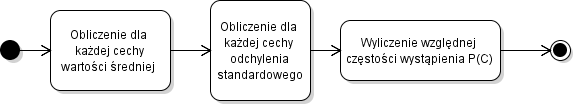
\includegraphics[scale = 0.5]{Obrazy/uczenie_schemat}
\caption{Schemat algorytmu uczenia klasyfikatora.}
\label{fig:obrazek k}
\end{figure}

Kolejny etap algorytmu to już analiza danych, które mają zostać sklasyfikowane. Polega ona wyliczeniu dla każdej cechy funkcji gęstości prawdopodobieństwa, ponieważ wszystkie cechy które będą wchodziły w skład obiektu będą cechami ciągłymi. Funkcja ta obliczana jest dla każdej klasy. Następnie w celu otrzymania prawdopodobieństwa $P(X|C_{i})$P(X|Ci) otrzymane wartości wymnaża się. Obiekt zostanie zakwalifikowana do klasy, w której obliczone prawdopodobieństwo $P(X|C_{i})$ jest najwyższe.  Rysunek 12 przedstawia algorytm przypisana klasy do zestawu cech.
\begin{figure}[h]
\centering
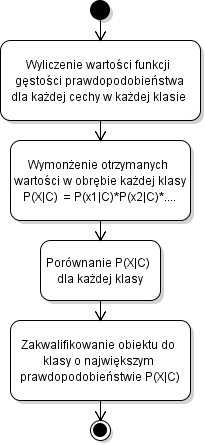
\includegraphics[scale = 0.6]{testowanie_schemat}
\caption{Schemat algorytmu przypisania klasy do obiektu.}
\label{fig:obrazek k}
\end{figure}

\subsection{Wykorzystanie klasyfikatora do rozpoznawania uderzeń serca}

W celu wstępnego wyznaczenia skuteczności algorytmu, przeprowadzono klasyfikacje na uderzeniach serca pochodzących z sygnału 100.dat i 228.dat z bazy danych MIT - BIH. Rodzaje uderzeń znajdujące się w tych sygnałach postanowiono podzielić na 3 klasy: 
\begin{itemize}
\item uderzenia normalne oznaczone literką \textit{N},
\item uderzenia komorowe oznaczone literą \textit{V},
\item inne uderzenia wyróżnione w bazie MIT - BIH.
\end{itemize}

Zdecydowano się na taki podział ponieważ dwie pierwsze grupy stanowią ponad 90\% wszystkich uderzeń serca występujących w całej bazie MIT-BIH.

\vspace{0.5cm}
Cechy jakie zostały zdefiniowane dla każdego obiektu to, zaproponowane na podstawie artykułu~\cite{1}:
\begin{itemize}
\item Pre interval RR - odległość miedzy aktualnym uderzeniem serca(analizowanym), a poprzednim uderzeniem serca,
\item Post inreval RR  - odległość między analizowanym uderzenie serca a kolejnym uderzeniem,
\item Average RR - średnia długość interwału RR dla całego analizowanego sygnału,
\item Ratio1 - stosunek pre RR interwal i post RR interval
\item Ratio2 - stosunek per interwalu do Avarage RR 
\end{itemize}

Dane zostały podzielone na dwie grupy treningową i testową odpowiednio w stosunku 4:1. Ilość obiektów w obu grupach łącznie wynosiło 4322, w grupie testowej było 864 próbek, a w treningowej 3458. Wynik klasyfikacji z wykorzystaniem wszystkich pięciu wcześniej opisanych cech. prezentuje Tabela~1.

\begin{table}[h]
\centering
\caption{Wynik klasyfikacji po zastosowaniu klasyfikatora Bayesa.}
    \begin{tabular}
{|l|c|c|c|}
    \hline
    ~              & Dobrze rozpoznane & Źle rozpoznane &  Dobrze rozpoznane/całość klasy \\ \hline
    Uderzenia N    & 776                      & 8                          & 0,99                     \\ \hline
    Uderzenia V    & 71                        & 1                          & 986                         \\ \hline
    Inne uderzenia & 4                       & 4                           & 0,5                     \\ \hline
    Suma           & 851                      & 13                          & 0,985                     \\ \hline
    \end{tabular}
\end{table}
 
Postanowiono sprawdzić jaka będzie skuteczność klasyfikacji, jeżeli uwzględnionych zostanie mniej cech. Na przykład cechy Ratio1 i Ratio2 są powiązane z przednimi cechami, więc istnieje podejrzenie, że skuteczność klasyfikatora z pominięciem tych cech może być wyższa zgodnie z naiwnym założeniem twierdzenia Bayesa. Okazało się jednak, że najlepszą skuteczność jakią można było uzyskać z wykorzystaniem tych cechy była w momencie nie uwzględniania ostatniej cechy Ratio2. Wyniki jakie otrzymano korzystający tylko pierwszych 4 cech (post i pre interval RR,average RR i Ratio1) znajdują się w Tabeli~2. 

\begin{table}[h]
\centering
\caption{Wynik klasyfikacji po zastosowaniu klasyfikatora Bayesa z wykorzystaniem 3 cech.}
    \begin{tabular}
{|l|c|c|c|}
    \hline
    ~              & Dobrze rozpoznane & Źle rozpoznane &  Dobrze rozpoznane/całość klasy \\ \hline
    Uderzenia N    & 785                      & 0                          & 1                     \\ \hline
    Uderzenia V    & 72                       & 0                           & 1                         \\ \hline
    Inne uderzenia & 0                       & 7                           & 0 \\ \hline
    Suma           & 857                      & 7                          & 0,992                   \\ \hline
    \end{tabular}
\end{table}

Można zauważyć, że w momencie skorzystania z mniejszej liczby cech skuteczność całego klasyfikatora wzrosła, jednak skuteczność w obrębie klas jest już bardzo różnorodna. Wszystkie uderzenia normalne i nadkomorowe występujące w grupie testowej zostały właściwie rozpoznane, jednak żadne z innych uderzeń nie zostało poprawnie sklasyfikowane. Powodem może być duża różnorodność wartości w obrębie tej klasy. Natomiast korzystając z wszystkich wyznaczonych cech, skuteczność poprawnego zaklasyfikowania do innych uderzeń jest znacznie większa i wynosi 50\%. Jednak w obu przypadkach skuteczność rozpoznania utrzymuje się na wysokim poziomie. Klasyfikator jest bardzo prosty w implementacji klasyfikacja przebiega bardzo sprawnie. O skuteczności algorytmu nie decyduje ilość danych treningowych tylko ich reprezentatywność. 
Klasyfikator Bayesa jest tak skonstruowany, że jednie czym można manipulować, aby polepszyć wyniki to zbiór treningowy - ilość i  rodzaj cech danego uderzenia, natomiast ilość danych w zbiorze treningowym nie jest już tak bardzo istotna.

\begin{thebibliography}{99}
\bibitem{aa} Wykład: Klasyfikacja, Naiwny klasyfikator Bayesa
\\\texttt{http://wazniak.mimuw.edu.pl}
\bibitem{1} K.M.~Senapati:
\emph{Automatic Classification of Heartbeats Using ECG Morphology and Heartbeat Interval Features}, Electrical Engineering IIT, 2014

\end{thebibliography}


\newpage
\section{Porównanie algorytmów}



\begin{table}[h]
\centering
\caption{Skuteczność klasyfikacji}
\label{accuracyTable}
\begin{tabular}{|l|l|l|l|l|}
\hline
kNN + ENN & Linear SVM & SVM + RBF & Naive Bayes & LDA \\ \hline
          & 76\%       & 99\%      & 96\%        &     \\ \hline
\end{tabular}
\end{table}

\begin{table}[h]
\centering
\caption{Czasy uczenia i klasyfikacji}
\label{timesTable}
\begin{tabular}{l|l|l|l|l|l|}
\cline{2-6}
                                        & kNN + ENN & Linear SVM & SVM + RBF & Naive Bayes & LDA \\ \hline
\multicolumn{1}{|l|}{Czas uczenia}      &           &  $8517\: ms$   &   $13481\: ms$   &   $21.9034\: ms$ & $15\: ms$    \\ \hline
\multicolumn{1}{|l|}{Czas klasyfikacji} &           &   $1\: ms$  &      $79\: ms$     &     $29.2936\: ms$        & $< 1\: ms$  \\ \hline
\end{tabular}
\end{table}

Testy wykonano na komputerze wyposażonym w procesor Intel Core i5-4200H o taktowaniu $2.80 \: GHz$ oraz 8 $Gb$ RAM w systemie operacyjnym Windows 10 64-bit.

\end{document}